
\chapter*{Introduzione}

La chimica quantistica è un campo che unisce la meccanica quantistica e la chimica per comprendere e prevedere il comportamento delle molecole e dei materiali. Uno degli strumenti più potenti in questo ambito è rappresentato dalle simulazioni, che consentono di prevedere proprietà molecolari senza la necessità di esperimenti fisici laboriosi e costosi \cite{IBMQuantum}. Tuttavia, l’efficacia di queste simulazioni è spesso limitata dalla crescita esponenziale della complessità computazionale con l’aumentare delle dimensioni del sistema, rendendole irrisolvibili anche per i supercomputer più avanzati.

In questo contesto, il calcolo quantistico si propone come un paradigma rivoluzionario. A partire dalle intuizioni di Feynman \cite{feynman_1982}, che suggerì di utilizzare sistemi quantistici per esplorare le proprietà della natura su scala quantistica, sono stati sviluppati dispositivi e algoritmi in grado di affrontare le limitazioni classiche. I \textbf{computer quantistici}, sfruttando fenomeni come la sovrapposizione, l’entanglement e l’interferenza, offrono una scalabilità potenzialmente superiore per risolvere problemi complessi, inclusi quelli relativi alla struttura elettronica delle molecole \cite{Cao_2019}. Questi progressi potrebbero trasformare non solo la chimica teorica, ma anche applicazioni come la farmacologia, la scienza dei materiali e le tecnologie energetiche \cite{Daley_2022,weidman_2024}.
Le simulazioni quantistiche renderebbero possibile la progettazione di nuovi composti e \textbf{materiali} con proprietà fisiche innovative e caratteristiche migliorate, come maggiore durata, leggerezza e costi ridotti. Ciò aprirebbe la strada a tecnologie all’avanguardia, come batterie più efficienti e sostenibili, dotate di maggiore capacità di immagazzinamento energetico, tempi di ricarica più rapidi e un minore impatto ambientale \cite{Zini_2023_battery}.
In \textbf{farmacologia}, la capacità di simulare con precisione il comportamento molecolare e le reazioni biochimiche offre una prospettiva rivoluzionaria per velocizzare lo sviluppo di farmaci e trattamenti salvavita. Attività di ricerca e validazione che oggi richiedono anni di sperimentazioni potrebbero essere drasticamente abbreviate, grazie alla possibilità di selezionare molecole promettenti con maggiore precisione e prevederne l’efficacia \cite{Johnson_2014,Pal_2024}.
Nel contesto industriale, il calcolo quantistico potrebbe rappresentare la chiave per rendere i \textbf{processi chimici} più sostenibili, mitigando la produzione di sottoprodotti dannosi e identificando soluzioni alternative. Ad esempio, il design di \textbf{catalizzatori} innovativi potrebbe portare a processi più efficienti per sostituire i derivati petrolchimici con materiali ecocompatibili o ottimizzare la cattura e la conversione del carbonio, un aspetto cruciale nella lotta contro il cambiamento climatico \cite{Paudel_2022,Reiher_2017}.
Inoltre, la possibilità di prevedere con precisione i \textbf{livelli energetici} di semiconduttori e altri materiali elettronici avanzati favorirebbe la ricerca nella microelettronica, portando allo sviluppo di dispositivi più performanti ed efficienti \cite{Wang_2024}.

\begin{figure}[H]
    \centering
    \begin{minipage}{\linewidth}
        \centering
        %\hspace{-0.2cm}
        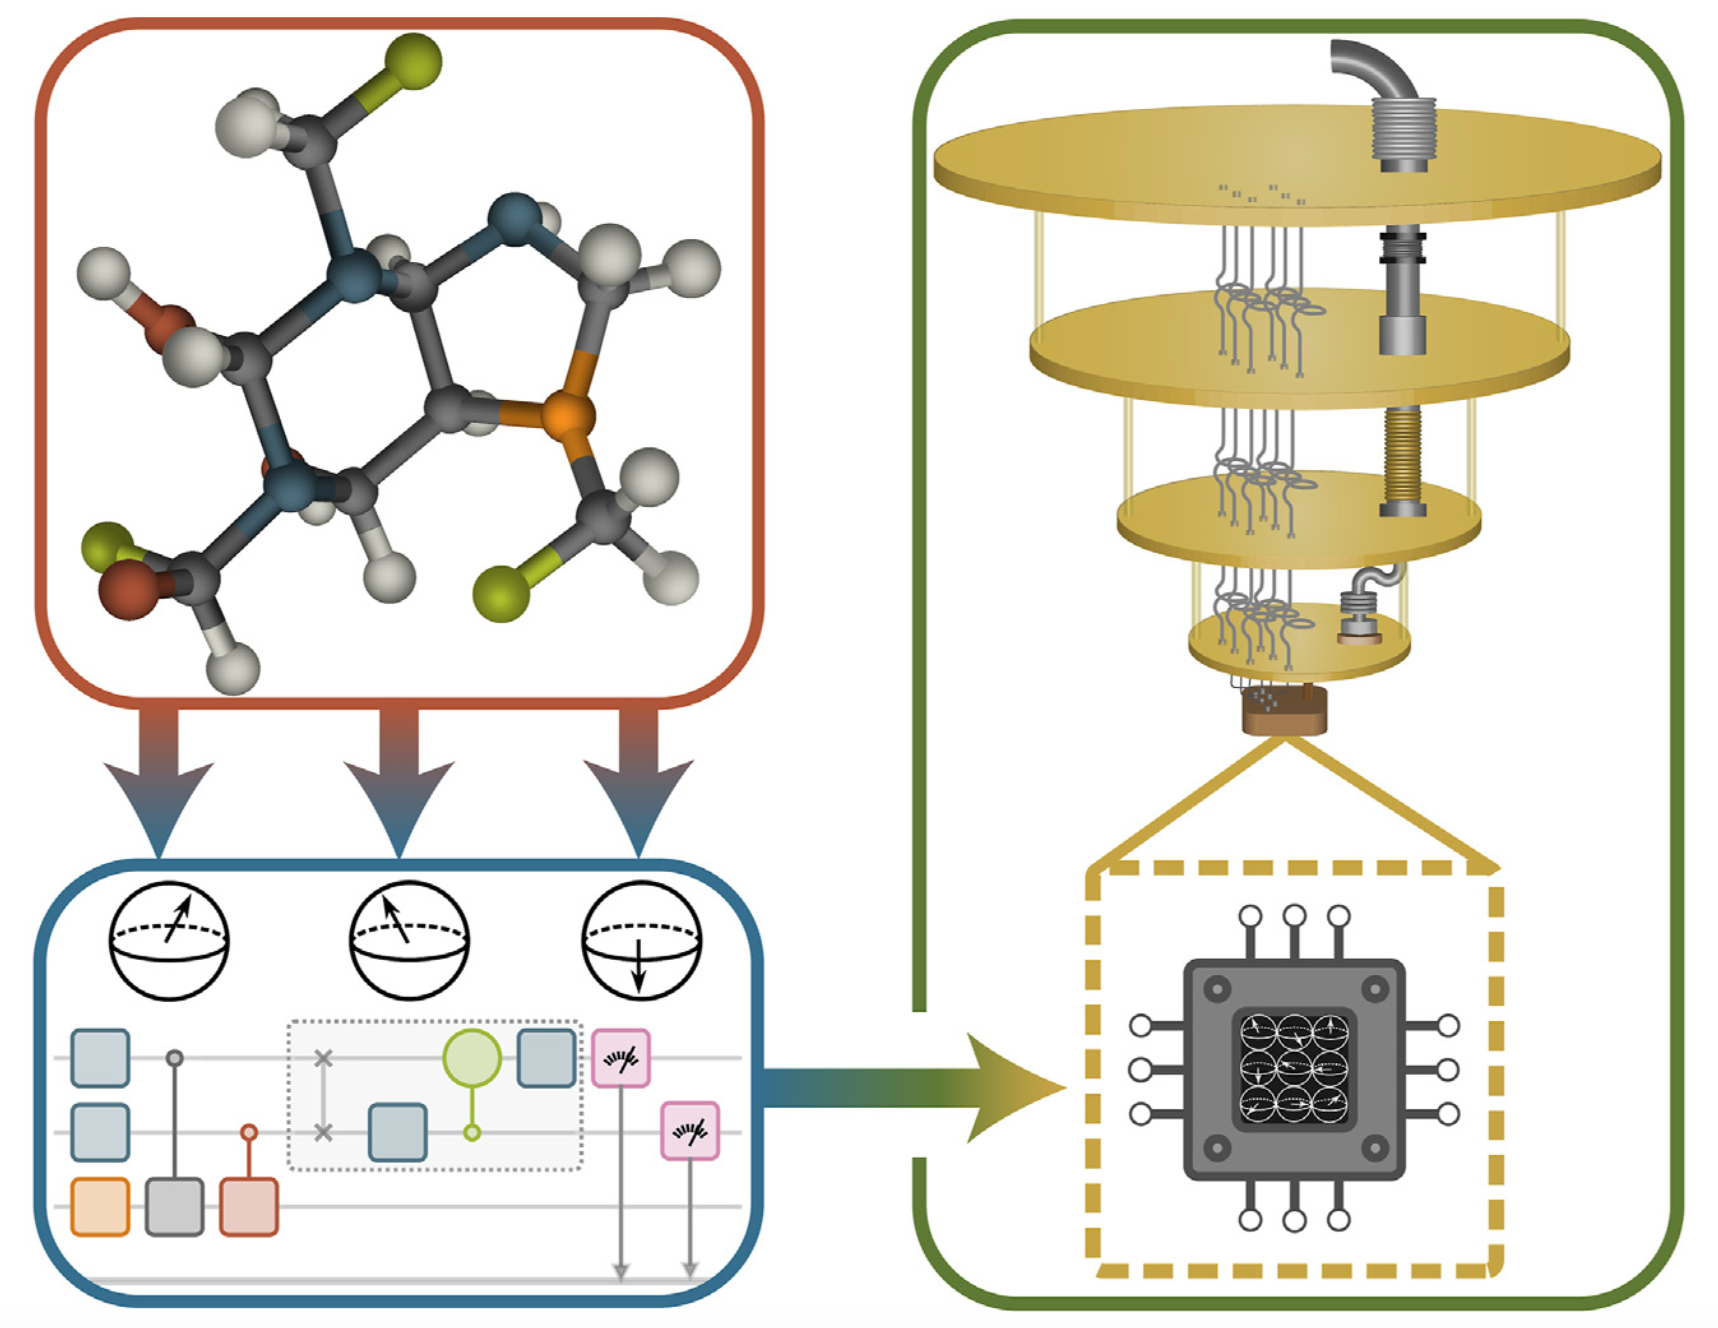
\includegraphics[width=.5\linewidth]{Immagini/Capitolo_0/qpu_chemistry.png}
        \caption{Illustrazione di una simulazione di chimica su quantum computer \cite{weidman_2024}.}
        \label{fig:qpu-chemistry}
    \end{minipage} \\[1ex]
    \begin{minipage}{.854\linewidth}
        \footnotesize
        Per calcolare una proprietà del sistema molecolare d'interesse (in alto a sinistra) si sceglie un metodo di calcolo, rappresentato con un diagramma (in basso a sinistra) che raffigura le operazioni quantistiche da svolgere su un set di qubit. Una volta costruito, il circuito quantistico è inviato ad un processore quantistico (a destra), contenuto all'interno di un criostato a temperature vicine ai 10 mK.
    \end{minipage}
\end{figure}

Un caso emblematico di difficoltà per la chimica computazionale classica è il calcolo delle interazioni elettroniche in molecole complesse. Descrivere il comportamento degli elettroni richiede approssimazioni che, spesso, sacrificano la precisione per contenere i costi computazionali. Al contrario, i computer quantistici - almeno in linea teorica - possono risolvere problemi che richiederebbero risorse esponenziali su hardware classico, anche utilizzando i migliori algoritmi disponibili.

Tuttavia, le implementazioni fisiche di questi dispositivi sono ancora in una fase embrionale e non sono ancora in grado di superare i computer classici in applicazioni pratiche. Nonostante ciò, in questo periodo caratterizzato da limiti hardware - spesso definito \textbf{era NISQ} (\inglese{Noisy Intermediate-Scale Quantum}) - lo sviluppo di software quantistico applicato alla chimica è un settore di ricerca in rapida evoluzione. Una delle direzioni più promettenti per rendere i calcoli quantistici applicabili alla simulazione di sistemi chimici nell'era NISQ è lo sviluppo di algoritmi \textbf{ibridi} che combinano metodi classici e quantistici.

Il \inglese{Variational Quantum Eigensolver} (VQE) \cite{Peruzzo_2014} rappresenta un esempio di approccio ibrido, progettato per adattarsi alle limitazioni tecnologiche dell’era NISQ. Il VQE sfrutta circuiti quantistici per stimare l’energia di stato fondamentale di un sistema molecolare, combinando simulazioni quantistiche e ottimizzazioni classiche. In questo lavoro, tale metodo è stato impiegato per confrontare differenti configurazioni di \textbf{ansatze}, con un’analisi comparativa delle loro prestazioni.

Resta da sottolineare che gli algoritmi quantistici appartengono a una classe differente e dovrebbero essere valutati attraverso metriche che non hanno un diretto analogo classico. Tra queste, ad esempio, ci sono la larghezza del circuito (numero di qubit), la profondità del circuito (numero di livelli di operazioni non commutanti) e il numero di misurazioni necessarie per ottenere quantità utili. 

In conclusione, le simulazioni di chimica quantistica, illustrate in Figura~\ref{fig:qpu-chemistry}, non solo rappresentano uno strumento avanzato per studiare le proprietà molecolari, ma costituiscono anche una piattaforma per testare le tecnologie quantistiche emergenti. Queste applicazioni permettono di esplorare i limiti attuali del calcolo quantistico, aprendo nuove opportunità per affrontare sfide scientifiche e tecnologiche di primaria importanza.

L’elaborato è strutturato per fornire un quadro d'insieme essenziale alla comprensione del metodo VQE e del suo contesto applicativo. Si parte dall’analisi dei concetti fondamentali della chimica computazionale classica, quindi si introducono i principi della computazione quantistica. Questo percorso teorico prepara il terreno per l’analisi delle simulazioni e dei risultati ottenuti, affrontati nelle sezioni successive.